% =====================================================================
%  6 Results III: steering (RQ3, second half)
%  Sources: reports/v3_runC_results.md (all sections),
%  reports/v3_identity_vs_baseline.md 1 (calibrated comparison),
%  S/results/v3/analysis/steering_summary.csv, steering_vs_trivial.csv,
%  steering_plus_shift_cv.csv. Figure: S/figures/v3/steering_dose_response.png
%  (made by S/fig_steering_v3.py; for the thesis consider removing the
%  in-figure title, since the caption carries it).
% =====================================================================
\section{Results III: Steering the Identity Effect}
\label{sec:steering}

% ---------------------------------------------------------------------
\subsection{Steering meets the criterion, and so does a constant shift}
\label{sec:steering:main}
% - Dampeners and text steering cut the distance by more than half;
%   dose-dependent; random heads do nothing -> causal.
% - No method beats the constant shift, because the models over-flag.
% - On top of a fitted shift, steering gains at most about 0.02
%   (Llama dampeners -0.015; Qwen text -0.016 / -0.022).
\fillin{Main steering result.}

\begin{table}[t]
  \centering
  \caption{Distance to the real group's share (\cref{eq:distance}), framed prompts (regions and
    gender), \variant{prefix}, held-out split B. Lower is better.}
  \label{tab:steering}
  \src{v3\_runC\_results.md §1}
  \begin{tabular}{lcc}
    \toprule
                                                     & \llamashort & \qwenshort \\
    \midrule
    unsteered                                        & 0.50 & 0.67 \\
    dampener heads, $k=100$                          & 0.22 & 0.43 \\
    text steering, $k=100$                           & 0.20 & 0.20 \\
    random heads, $k=100$                            & 0.50 & 0.66 \\
    activation steering (framing direction removed)  & 0.38 & 0.66 \\
    \midrule
    constant shift (fitted on split A)               & 0.19 & 0.22 \\
    \bottomrule
  \end{tabular}
\end{table}

\begin{figure}[t]
  \centering
  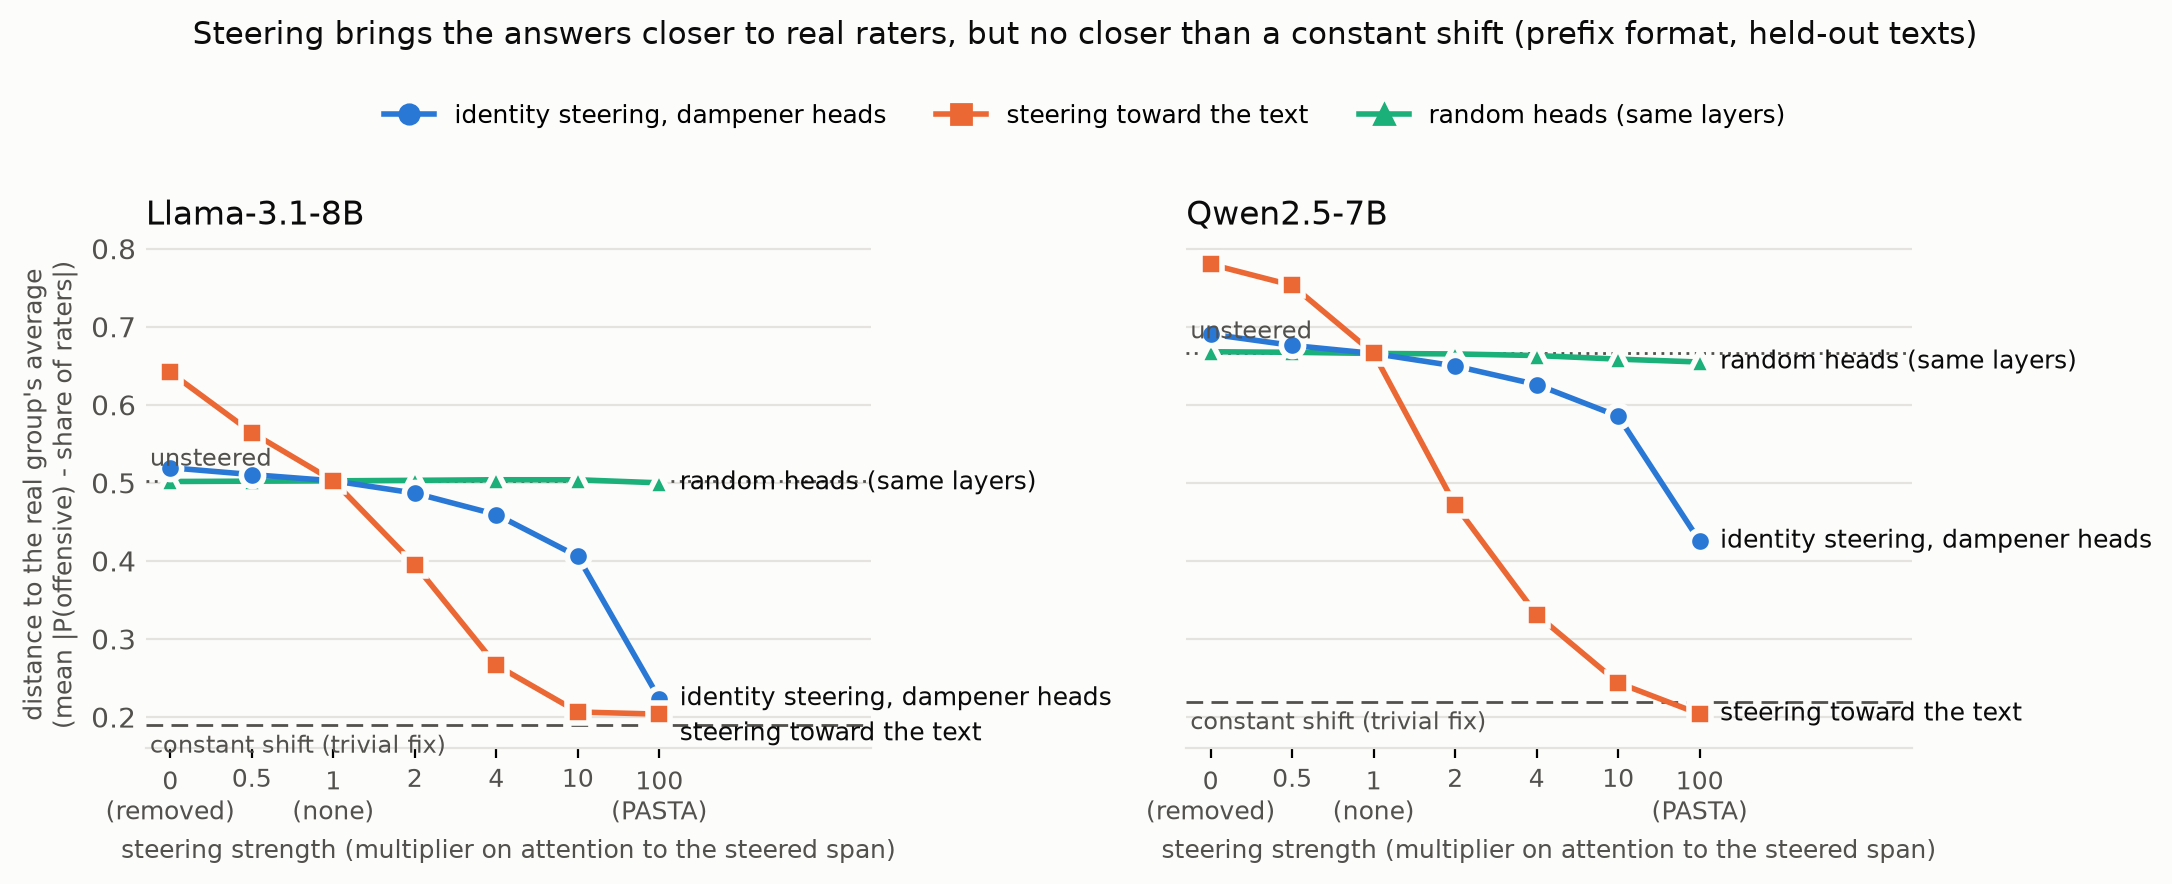
\includegraphics[width=\linewidth]{v3/steering_dose_response.png}
  \caption{Distance to the real group's average rating as a function of steering strength
    (\variant{prefix}, held-out texts). \fillin{Finish caption.}}
  \label{fig:dose-response}
\end{figure}

% ---------------------------------------------------------------------
\subsection{What each method actually does}
\label{sec:steering:methods}
% - Text steering: -5 to -6 log-odds on every prompt incl. unframed; flags
%   0-3% of texts; ranking drops (Llama Spearman 0.13 -> 0.03).
% - Dampeners (Llama): regions -2.5, placebos +1.7, place names +0.6;
%   ranking kept (0.15 -> 0.18); flagged 75% -> 24%. Cleanest
%   identity-specific intervention. Qwen: regions -5.0, placebos -1.5,
%   place -3.4 (partly specific). Not in target.
% - Amplifiers: Qwen regions +4.1, distance +0.09; Llama -0.1.
% - Gender / religion: region dampeners move them much less (-0.7, -0.5).
% - Activation steering: Llama regions -1.4, placebos unchanged; Qwen ~0.
\fillin{Per-method analysis: specificity, ranking, flag rate.}

% Optional table: change in log-odds for region / placebo / place under
% each method (from steering_summary.csv).

% ---------------------------------------------------------------------
\subsection{Alignment versus calibration}
\label{sec:steering:calibration}
% - Relative alignment under steering: rho -0.04 to +0.03 everywhere.
% - Calibrated comparison (table below): after the same constant shift,
%   framing adds nothing (Llama) or hurts (Qwen); predicting each group
%   with the all-raters share is twice as close (0.10).
\fillin{Separating calibration from alignment.}

\begin{table}[t]
  \centering
  \caption{Distance to the real group's share before and after the same constant shift
    (fitted on one half of the texts, evaluated on the other).}
  \label{tab:calibrated}
  \src{v3\_identity\_vs\_baseline.md §1}
  \begin{tabular}{lcccc}
    \toprule
    & \multicolumn{2}{c}{\llamashort} & \multicolumn{2}{c}{\qwenshort} \\
    \cmidrule(lr){2-3}\cmidrule(lr){4-5}
                                       & \variant{prefix} & \variant{infix} & \variant{prefix} & \variant{infix} \\
    \midrule
    unframed, raw                      & 0.34 & 0.34 & 0.42 & 0.42 \\
    framed, raw                        & 0.50 & 0.49 & 0.67 & 0.58 \\
    unframed + constant shift          & 0.19 & 0.20 & 0.20 & 0.20 \\
    framed + constant shift            & 0.19 & 0.19 & 0.24 & 0.23 \\
    dampener-steered + constant shift  & 0.17 & 0.19 & 0.22 & 0.22 \\
    \midrule
    all raters' share as prediction    & \textbf{0.10} & \textbf{0.10} & \textbf{0.10} & \textbf{0.10} \\
    \bottomrule
  \end{tabular}
\end{table}
